\documentclass{article}

\usepackage{postprocess/context/arxiv}

\usepackage[utf8]{inputenc} % allow utf-8 input
\usepackage{amsmath}
\usepackage[T1]{fontenc}    % use 8-bit T1 fonts
\usepackage{hyperref}       % hyperlinks
\usepackage{url}            % simple URL typesetting
\usepackage{booktabs}       % professional-quality tables
\usepackage{amsfonts}       % blackboard math symbols
\usepackage{nicefrac}       % compact symbols for 1/2, etc.
\usepackage{microtype}      % microtypography
\usepackage{graphicx}
\usepackage{natbib}
\usepackage{doi}
\usepackage{float}
\usepackage{subcaption}
\usepackage{wrapfig}

\title{Causal Discovery Report on Abalone}

\author{ \href{https://orcid.org/0000-0000-0000-0000}{
\includegraphics[scale=0.06]{postprocess/context/orcid.pdf}\hspace{1mm}Causal Copilot}}

\renewcommand{\headeright}{Technical Report}
\renewcommand{\undertitle}{Technical Report}

\hypersetup{
pdftitle={Causal Discovery Report on Abalone},
pdfauthor={Causal Copilot},
pdfkeywords={Causal Discovery, Large Language Model, PC, Abalone},
}

\begin{document}
\maketitle

\begin{abstract}
This report conducts a causal discovery analysis on a dataset concerning abalones, marine mollusks of notable biological and economic importance. The dataset includes various physical metrics such as age, length, diameter, height, and different weight measurements. A comprehensive causal discovery process was implemented utilizing the PC, GES, and DirectLiNGAM algorithms, guided by a large language model for both algorithm selection and hyperparameter tuning. The results indicate intricate causal relationships: age significantly impacts diameter and viscera weight, while length influences shell and shucked weight, illustrating the interplay between these variables. Notably, shell weight demonstrates reciprocal effects on other dimensions, suggesting feedback mechanisms in growth patterns. While certain statistical edges indicate high confidence, inconsistencies in expert knowledge highlight the need for careful interpretation. Our contribution lies in refining the understanding of abalone biology and providing a framework for future causal analyses in ecological and economic contexts.
\end{abstract}

\keywords{Causal Discovery, Large Language Model, PC, Abalone}

\raggedbottom
\section{Introduction}
The dataset under examination pertains to abalones, marine mollusks renowned for their unique biological characteristics and commercial significance. It encompasses various physical metrics, including age, length, diameter, height, and different weight measurements—whole, shucked, viscera, and shell. Age serves as a key determinant of the abalone's growth, influencing its size and weight, while the physical dimensions are vital indicators of overall health and market viability. Understanding the potential causal relationships among these variables offers insights into the growth patterns and biological mechanisms of abalones, which is essential not only for fisheries management but also for sustaining the commercial value of this species. This report aims to explore the causal relationships represented in the dataset, contributing to a deeper understanding of abalone biology and its implications in ecological and economic contexts.

\section{Background Knowledge}
\subsection{Detailed Explanation about the Variables}
\begin{itemize}
\item \textbf{Age}: This variable typically represents the age of the abalone, which is usually estimated based on the ring count on the shell. It is crucial for understanding the growth and maturity of the abalone.
\item \textbf{Length}: This is the measurement of the abalone's longest dimension. It serves as an important indicator of the size and growth stage of the abalone.
\item \textbf{Diameter}: This variable measures the width of the abalone, perpendicular to the length. It provides additional information about the physical size and shape of the abalone.
\item \textbf{Height}: This represents the vertical measurement (or thickness) of the abalone. Height can influence how much volume the abalone has, thereby affecting its weight and overall growth.
\item \textbf{Whole weight}: This is the total weight of the abalone, encompassing all parts (shell, meat, etc.). It is a significant measurement from a commercial perspective since it directly relates to the market value.
\item \textbf{Shucked weight}: This variable indicates the weight of the abalone once the shell is removed, focusing on the edible portion. It is particularly important for assessing the portion of the abalone that can be sold.
\item \textbf{Viscera weight}: This measures the weight of the internal organs of the abalone after shucking. This information is relevant for understanding the biological makeup and potential edible portions of the abalone.
\item \textbf{Shell weight}: This represents the weight of the abalone's shell separately. It is important for understanding the structural components and health of the abalone.
\end{itemize}

\subsection{Possible Causal Relations among these Variables}
\begin{minipage}[t]{0.7\linewidth}
\begin{itemize}
    \item \textbf{Age $\rightarrow$ Length}: As abalones age, they tend to grow longer, indicating that older specimens are generally larger in terms of length.
    \item \textbf{Age $\rightarrow$ Diameter}: With maturation, abalones typically increase in diameter, as they develop a larger and more robust shell structure.
    \item \textbf{Age $\rightarrow$ Height}: Similar to length and diameter, the height of abalones increases with age, reflecting their overall growth and development.
    \item \textbf{Length $\rightarrow$ Whole weight}: Greater length contributes to increased mass, leading to a higher whole weight for the abalone.
    \item \textbf{Diameter $\rightarrow$ Whole weight}: An increase in diameter suggests a larger volume, which positively influences the whole weight of the abalone.
    \item \textbf{Height $\rightarrow$ Whole weight}: Height plays a critical role in determining the total volume, thereby affecting the whole weight.
    \item \textbf{Whole weight $\rightarrow$ Shucked weight}: The total weight of the abalone directly impacts the shucked weight, as a heavier abalone will yield more edible meat once the shell is removed.
    \item \textbf{Whole weight $\rightarrow$ Viscera weight}: The total weight is likely to correlate with the weight of internal organs, as heavier abalones generally have more substantial viscera.
    \item \textbf{Whole weight $\rightarrow$ Shell weight}: An increase in the whole weight of an abalone typically corresponds with a heavier shell, as both shell and body grow together.
    \item \textbf{Shucked weight $\rightarrow$ Viscera weight}: The proportion of the body that consists of edible meat resonates with the weight of the internal organs, indicating a relationship between these two weights. 
    \item \textbf{Shell weight $\rightarrow$ Age}: Older abalones may possess thicker and heavier shells, indicating a relationship between age and shell weight.
\end{itemize}
\end{minipage}
\hspace{0.05\textwidth}
\begin{minipage}[t]{0.3\linewidth}
    \begin{figure}[H]
        \centering
        \resizebox{\linewidth}{!}{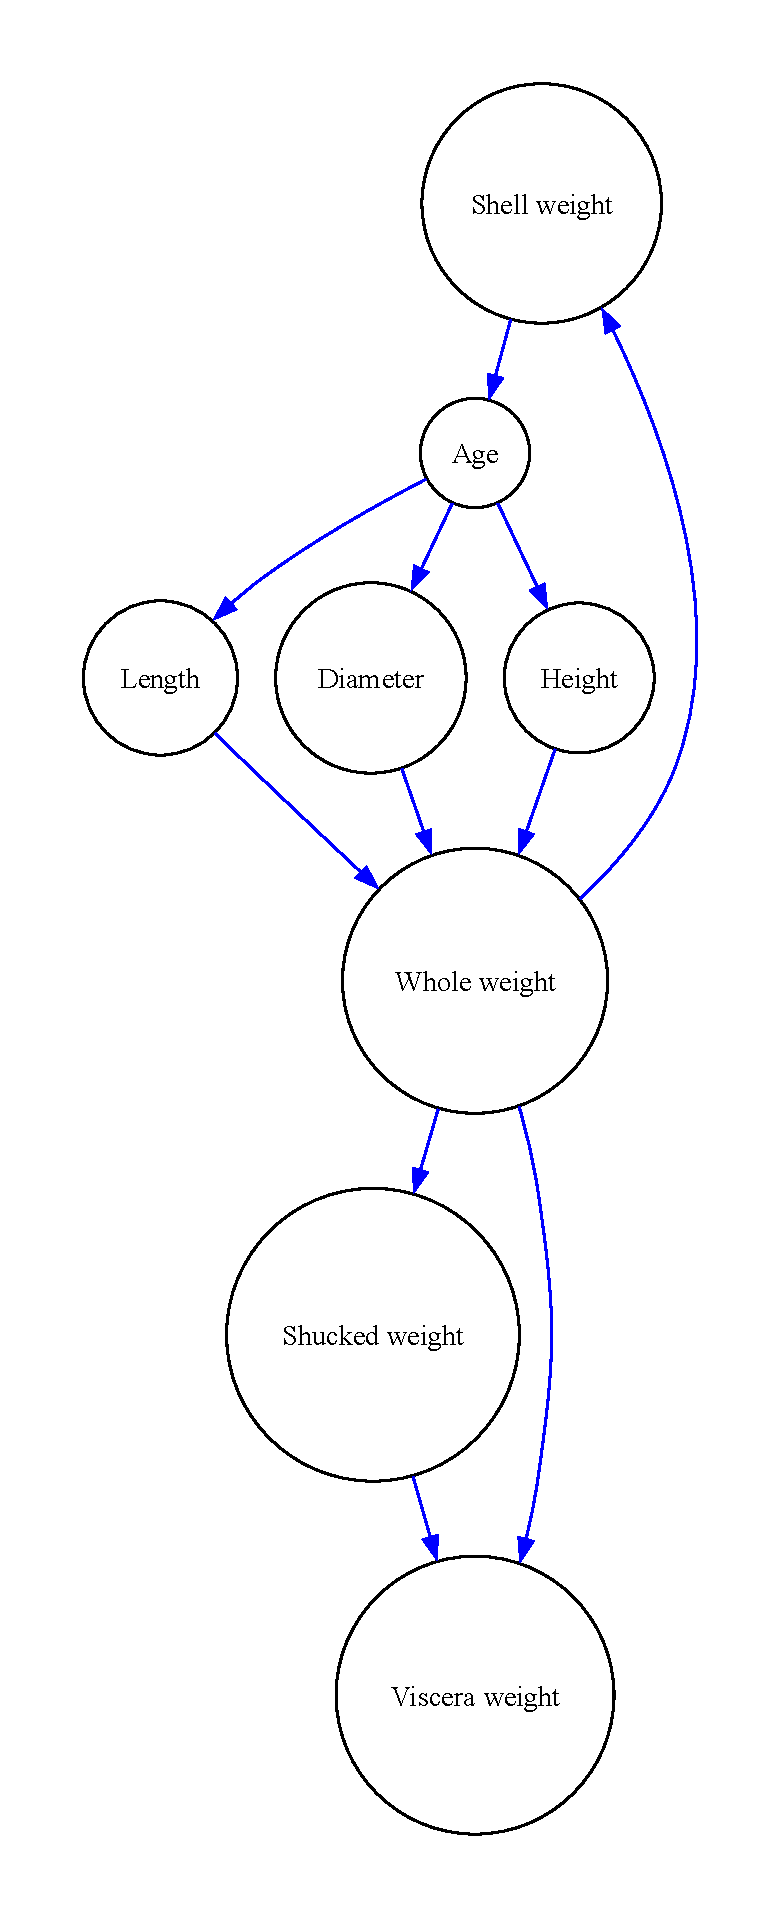
\includegraphics[height=0.4\textheight]{./demo_data/20241104_112841/Abalone/output_graph/potential_relation.pdf}}
        \caption{\label{fig:relation}Possible Causal Relation Graph}
    \end{figure}
\end{minipage}

\section{Dataset Descriptions and EDA}
The following is a preview of our original dataset.

\begin{table}[H]
    \centering
    \caption{Dataset Preview}
    \begin{tabular}{rrrrrrrr}
\toprule
 Age &  Length &  Shell weight &  Diameter &  Height &  Whole weight &  Shucked weight &  Viscera weight \\
\midrule
15.0 &   0.455 &         0.365 &     0.095 &  0.5140 &        0.2245 &          0.1010 &           0.150 \\
 7.0 &   0.350 &         0.265 &     0.090 &  0.2255 &        0.0995 &          0.0485 &           0.070 \\
 9.0 &   0.530 &         0.420 &     0.135 &  0.6770 &        0.2565 &          0.1415 &           0.210 \\
10.0 &   0.440 &         0.365 &     0.125 &  0.5160 &        0.2155 &          0.1140 &           0.155 \\
 7.0 &   0.330 &         0.255 &     0.080 &  0.2050 &        0.0895 &          0.0395 &           0.055 \\
\bottomrule
\end{tabular}
\end{table}

\subsection{Data Properties}
We employ several statistical methods to identify data properties.

The shape of the data, data types, and missing values are assessed directly from the dataframe. Linearity is evaluated using Ramsey’s RESET test, followed by the Benjamini \& Yekutieli procedure for multiple test correction. Gaussian noise is assessed through the Shapiro-Wilk test, also applying the Benjamini \& Yekutieli procedure for multiple test correction. Time-Series and Heterogeneity are derived from user queries.

Properties of the dataset we analyzed are listed below.

\begin{table}[H]
    \centering
    \caption{Data Properties}
    \begin{tabular}{rrrrrrr}
\toprule
Shape ($n$ x $d$) & Data Type & Missing Value & Linearity & Gaussian Errors & Time-Series & Heterogeneity \\
\midrule
(4177, 8)   & Continuous & False & False & False & False & False \\
\bottomrule
\end{tabular}
\end{table}

\subsection{Distribution Analysis}
The following figure shows distributions of different variables. The orange dash line represents the mean, and the black line represents the median. Variables are categorized into three types according to their distribution characteristics.

\begin{figure}[H]
\centering
\includegraphics[width=\linewidth]{./demo_data/20241104_112841/Abalone/output_graph/eda_dist.jpg}
\caption{\label{fig:dist}Distribution Plots of Variables}
\end{figure}

\begin{itemize}
\item Slight left skew distributed variables: Length, Shell weight, Diameter, Whole weight
\item Slight right skew distributed variables: Age, Height, Shucked weight, Viscera weight
\item Symmetric distributed variables: None
\end{itemize}

\subsection{Correlation Analysis}

\begin{minipage}[t]{0.5\linewidth}
In this analysis, we will categorize the correlation statistics of features in the dataset into three distinct categories: Strong correlations, Moderate correlations, and Weak correlations.

\begin{itemize}
\item Strong Correlated Variables: Shell weight and Length, Height and Whole weight, Shucked weight and Height, Viscera weight and Height, Shell weight and Viscera weight, Shucked weight and Shell weight, Shucked weight and Whole weight, Viscera weight and Shucked weight
\item Moderate Correlated Variables: Length and Age, Shell weight and Age, Diameter and Age, Height and Age, Shucked weight and Age, Viscera weight and Age, Diameter and Length, Diameter and Shell weight, Diameter and Height, Whole weight and Length, Whole weight and Diameter, Whole weight and Shell weight
\item Weak Correlated Variables: Height and Diameter, Whole weight and Age, Shucked weight and Diameter, Viscera weight and Diameter
\end{itemize}
\vfill
\end{minipage}
\hfill
\begin{minipage}[t]{0.5\linewidth}
    \begin{figure}[H]
        \centering
        \vspace{-1.5cm}
        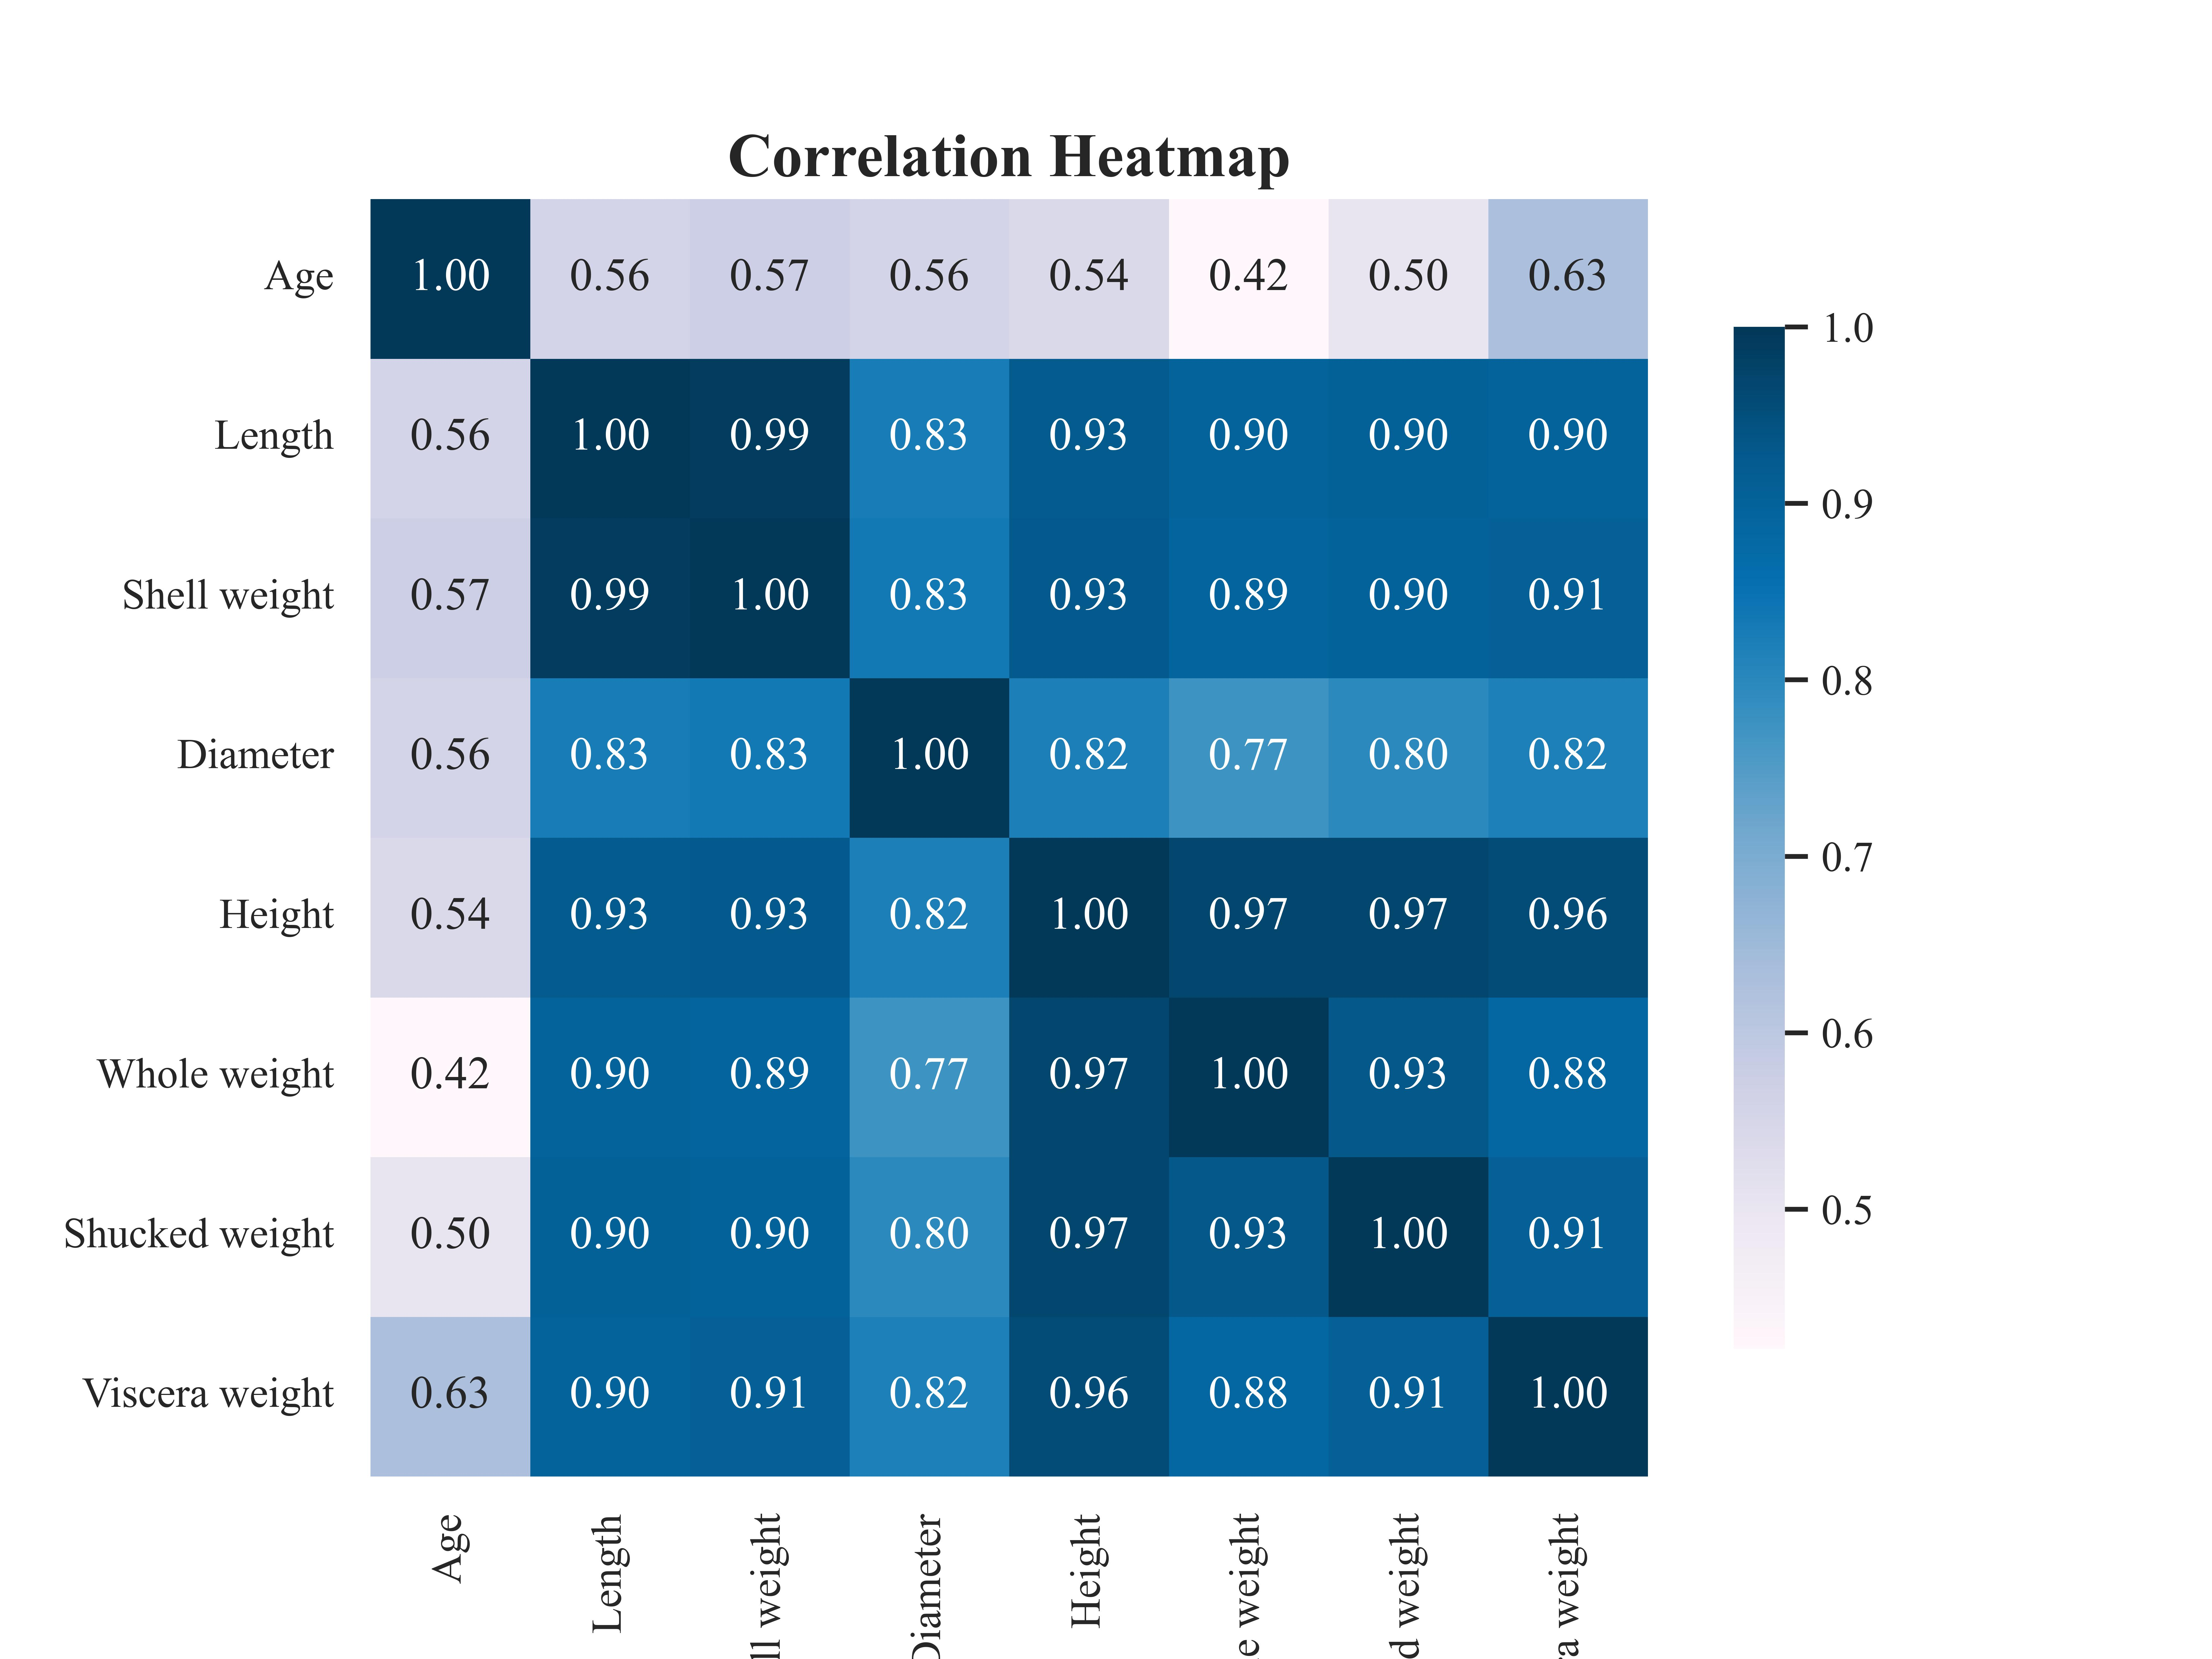
\includegraphics[width=\linewidth]{./demo_data/20241104_112841/Abalone/output_graph/eda_corr.jpg}
        \caption{\label{fig:corr}Correlation Heatmap of Variables}
    \end{figure}
\end{minipage}

\section{Discovery Procedure}

In this section, we provide a detailed description of the causal discovery process implemented by Causal Copilot. We also provide the chosen algorithms and hyperparameters, along with the justifications for these selections.

\subsection{Data Preprocessing}
In this initial step, we preprocessed the data and examined its statistical characteristics. This involved cleaning the data, handling missing values, and performing exploratory data analysis to understand distributions and relationships between variables.

\subsection{Algorithm Selection assisted with LLM}
Following data preprocessing, we employed a large language model (LLM) to assist in selecting appropriate algorithms for causal discovery based on the statistical characteristics of the dataset and relevant background knowledge. The top three chosen algorithms, listed in order of suitability, are as follows:   

\begin{itemize}
    \item \textbf{PC}:
    \begin{itemize}
        \item \textbf{Description}: The PC algorithm is a constraint-based method that learns the structure of a causal graph from data by testing conditional independencies between variables.
        \item \textbf{Justification}: Given the large sample size of 4177 and the characteristics of the data, PC is highly suitable as it efficiently handles large datasets where all relevant variables are observed, producing a Markov equivalence class.
    \end{itemize}

    \item \textbf{GES}:
    \begin{itemize}
        \item \textbf{Description}: Greedy Equivalence Search (GES) is a score-based causal discovery algorithm that identifies the optimal causal structure by navigating the space of equivalence classes of Directed Acyclic Graphs (DAGs).
        \item \textbf{Justification}: GES is appropriate due to its efficiency in navigating large and complex causal structures, especially when dealing with large sample sizes and assuming Gaussian errors, as the dataset exhibits non-Gaussian noise.
    \end{itemize}

    \item \textbf{DirectLiNGAM}:
    \begin{itemize}
        \item \textbf{Description}: DirectLiNGAM introduces an efficient, stepwise linear regression approach to directly estimate the causal order, useful for linear relationships with non-Gaussian noise.
        \item \textbf{Justification}: This algorithm is suitable because it assumes linear relationships and can handle non-Gaussian errors, thus fitting the dataset's characteristics where linearity is not predominant.
    \end{itemize}
\end{itemize}

\subsection{Hyperparameter Values Proposal assisted with LLM}
Once the algorithms were selected, the LLM aided in proposing hyperparameters for the chosen algorithm, which are specified below:

\begin{itemize}
    \item \textbf{alpha}:
    \begin{itemize}
        \item \textbf{Value}: 0.05
        \item \textbf{Explanation}: Given the larger sample size of 4177, using the default alpha value of 0.05 strikes a balance between Type I error control and the ability to detect true effects without being overly conservative. This value is appropriate since the sample is more than 500 and less than 10000.
    \end{itemize}

    \item \textbf{indep\_test}:
    \begin{itemize}
        \item \textbf{Value}: fisherz
        \item \textbf{Explanation}: Since the dataset consists of continuous variables, Fisher's Z test is suitable despite its assumptions of linearity and Gaussianity. It is the recommended method for independence testing in continuous datasets.
    \end{itemize}

    \item \textbf{depth}:
    \begin{itemize}
        \item \textbf{Value}: -1
        \item \textbf{Explanation}: Setting depth to -1 allows for unlimited depth in the adjacency search, which is useful given the eight variables in this dataset. Since the graph size is relatively small (8 nodes), unlimited depth would not significantly impact computation time and ensures comprehensive causal structure exploration.
    \end{itemize}
\end{itemize}

\subsection{Graph Tuning with Bootstrap and LLM Suggestion}
In the final step, we performed graph tuning with suggestions provided by the Bootstrap and LLM.

Firstly, we use the Bootstrap technique to get how much confidence we have on each edge in the initial graph. If the confidence probability of a certain edge is greater than 95\% and it is not in the initial graph, we force it. Otherwise, if the confidence probability is smaller than 5\% and it exists in the initial graph, we change it to the edge type with the highest probability.

After that, We utilize LLM to help us prune edges and determine the direction of undirected edges according to its knowledge repository. In this step LLM can use background knowledge to add some edges that are neglected by Statistical Methods. Voting techniques are used to enhance the robustness of results given by LLM, and the results given by LLM should not change results given by Bootstrap.

By integrating insights from both of Bootstrap and LLM to refine the causal graph, we can achieve improvements in graph's accuracy and robustness.

\section{Results Summary}

\subsection{Initial Graph}

\begin{figure}[H]
    \centering
    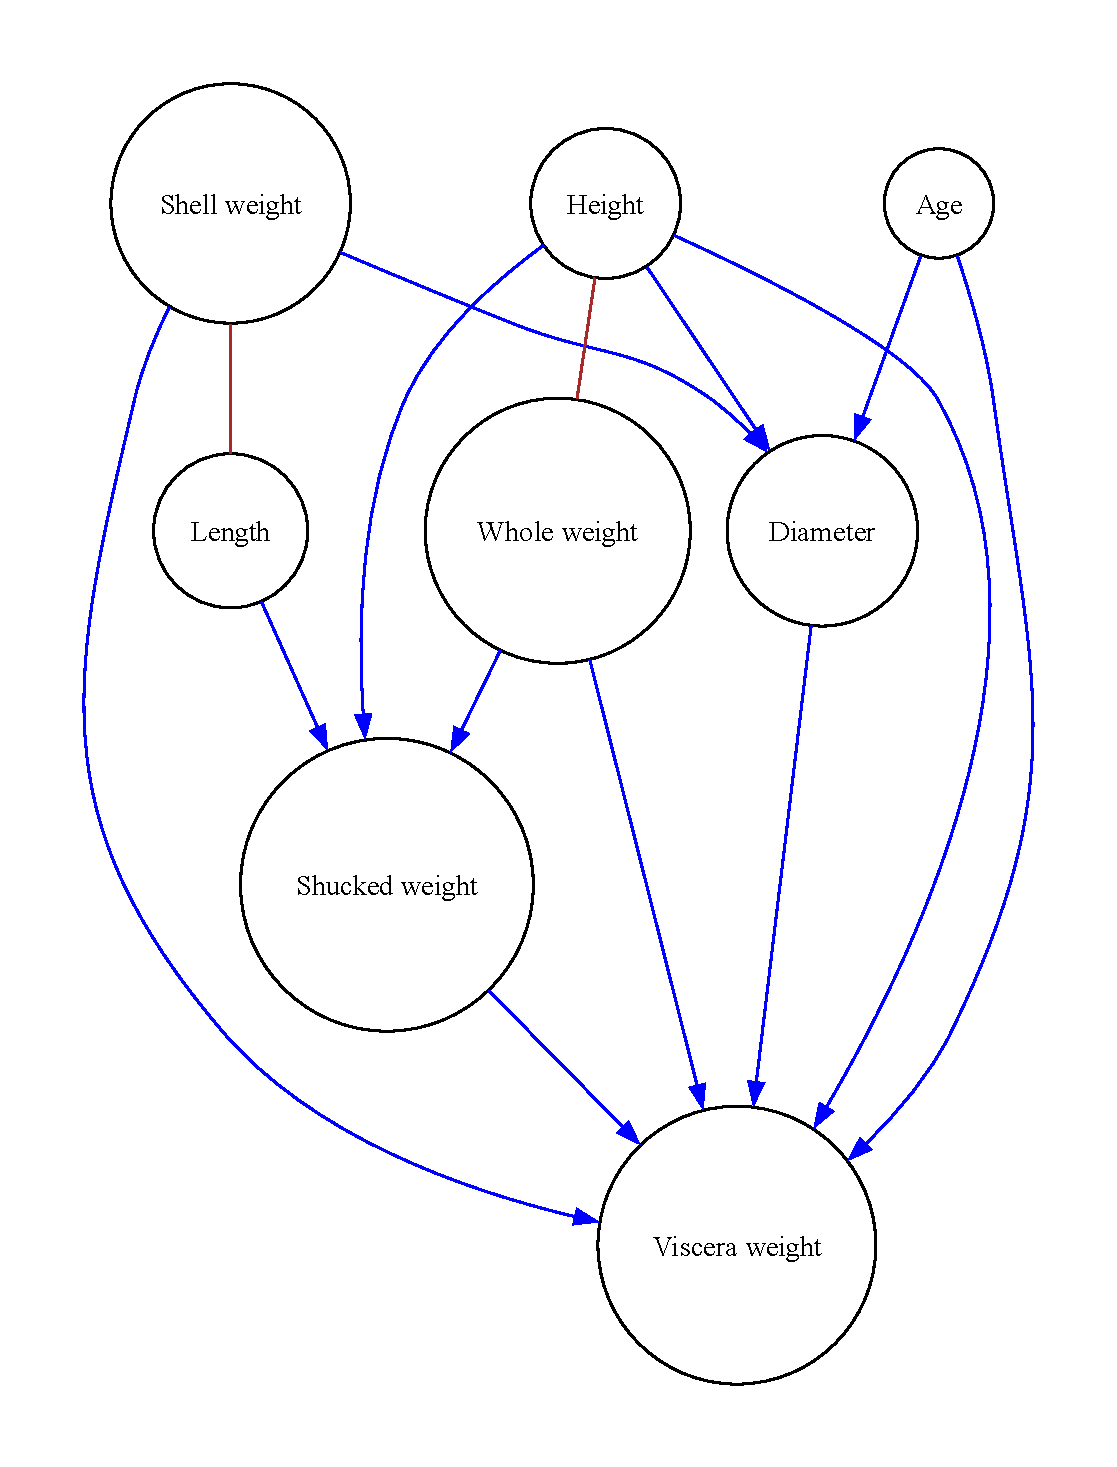
\includegraphics[height=0.4\textheight]{./demo_data/20241104_112841/Abalone/output_graph/initial_graph.pdf}
    \caption{Initial Graph}
\end{figure}

The above is the initial result graph produced by our algorithm.

The causal analysis reveals a complex interaction among various biological measurements. Age influences both Diameter and Viscera weight, suggesting that as an organism ages, its body size and internal weight components also increase. Length emerges as a significant factor, affecting Shell weight and Shucked weight; this indicates that larger lengths contribute to the growth of these associated traits. Interestingly, Shell weight also has reciprocal influences, notably affecting Length, Diameter, and Viscera weight, indicating a feedback loop where the size of the shell may influence overall morphology and internal weight. Height plays a crucial role as well, impacting Diameter, Whole weight, Shucked weight, and Viscera weight, suggesting that taller organisms are associated with increased overall mass and specific weights. Additionally, Whole weight reinforces its connection across various dimensions, causing Height, Shucked weight, and Viscera weight, thereby emphasizing the integral relationship between overall body mass and the growth of individual components, while Shucked weight directly affects Viscera weight, indicating that the processing or removal of certain parts has a direct implication on the internal weight metrics.

\subsection{Revised Graph}

\begin{minipage}[t]{0.6\linewidth}
By using the method mentioned in the Section 4.4, we provide a revise graph pruned with Bootstrap and LLM suggestion. Pruning results are as follows.

Bootstrap doesn't force or forbid any edges.

The following are force results given by LLM:

\begin{itemize}
    \item \textbf{Age $\rightarrow$ Length}: As abalones age, they tend to grow larger. Therefore, older abalones will generally have a greater length as a result of their natural growth process.
    \item \textbf{Age $\rightarrow$ Shell weight}: Older abalones typically exhibit heavier and possibly thicker shells, as shell weight increases with time due to growth and maturity.
    \item \textbf{Age $\rightarrow$ Height}: With aging, abalones increase in size including their vertical dimension; hence, older abalones are expected to have greater height.
    \item \textbf{Age $\rightarrow$ Whole weight}: Aging abalones generally tend to be heavier overall due to increased size and growth, resulting in a higher whole weight.
    \item \textbf{Age $\rightarrow$ Shucked weight}: As abalones grow older and larger, they also tend to have a higher shucked weight since more edible tissue develops with age.
    \item \textbf{Length $\rightarrow$ Diameter}: Generally, as the length of an abalone increases, the diameter also tends to increase, reflecting the overall growth in size.
    \item \textbf{Length $\rightarrow$ Height}: Longer abalones are likely to also be taller, resulting from proportional growth in their physical dimensions.
    \item \textbf{Length $\rightarrow$ Whole weight}: The overall length of the abalone directly contributes to its body mass, leading to a higher total whole weight.
    \item \textbf{Length $\rightarrow$ Viscera weight}: The visceral weight is expected to increase with length as larger abalones have more internal organs, thus affecting the overall viscera weight.
    \item \textbf{Shell weight $\rightarrow$ Whole weight}: The weight of the shell is part of the total body mass; hence, larger shell weights usually correspond to a greater whole weight.
    \item \textbf{Shell weight $\rightarrow$ Shucked weight}: The shell weight is linked to shucked weight since heavier shells often indicate more mass of the edible portion present in the abalone.
\end{itemize}

The following are directions of remaining undirected edges determined by the LLM:
\begin{itemize}
    \item \textbf{Length $\rightarrow$ Shell weight}: As abalones grow in length, their shells also typically increase in size and weight. Therefore, a larger length is expected to cause an increase in shell weight due to the physical growth of the abalone.
    \item \textbf{Height $\rightarrow$ Whole weight}: The height of an abalone contributes to its overall body mass, as a taller shell can support a greater volume of meat. Thus, an increase in height is likely to influence an increase in whole weight.
\end{itemize}

This structured approach ensures a comprehensive and methodical analysis of the causal relationships within the dataset.
\vfill
\end{minipage}
\hfill
\begin{minipage}[t]{0.4\linewidth}
    \begin{figure}[H]
        \centering
        \vspace{-0.5cm}
        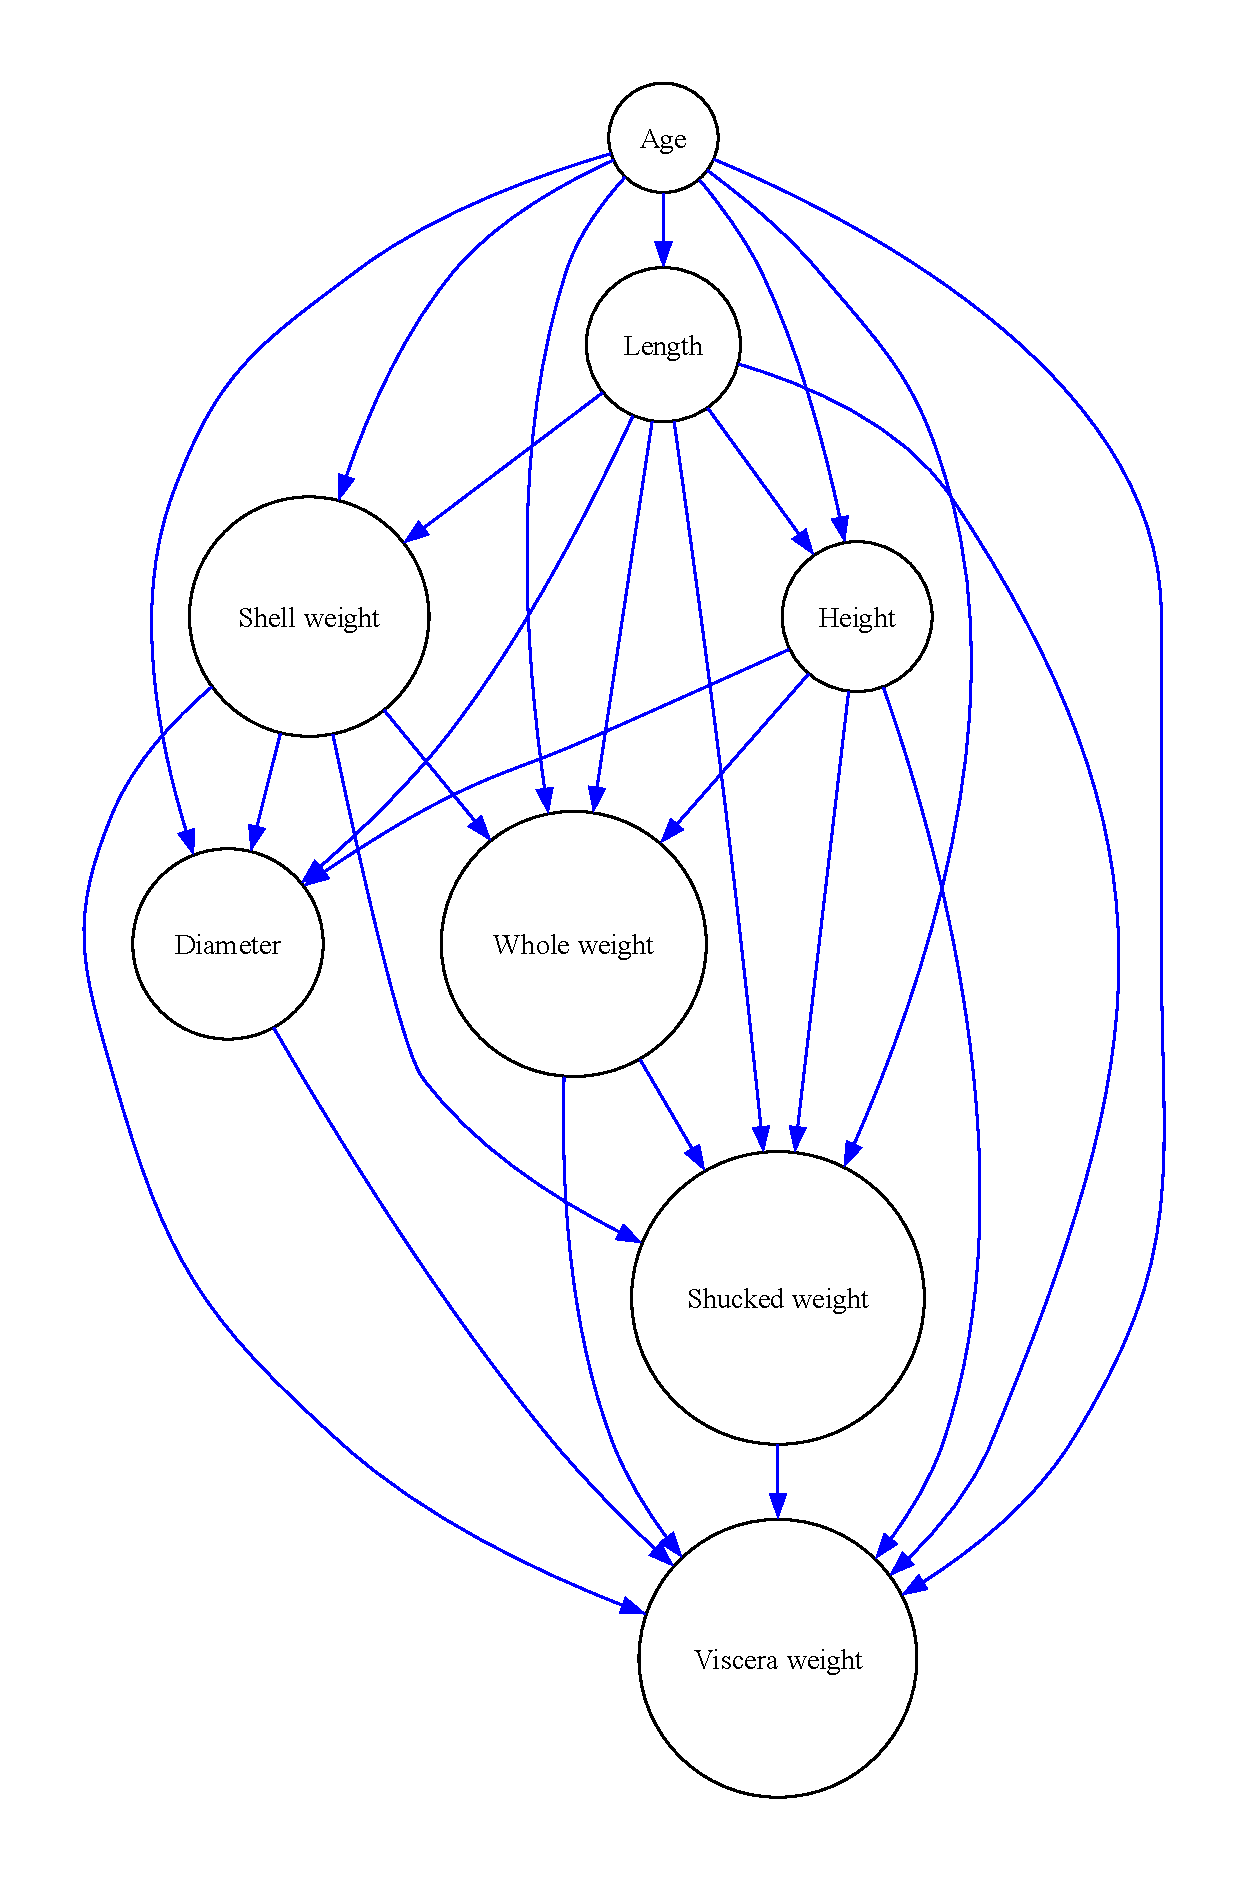
\includegraphics[width=\linewidth]{./demo_data/20241104_112841/Abalone/output_graph/revised_graph.pdf}
        \caption{\label{fig:corr}Revised Graph}
    \end{figure}
\end{minipage}

\subsection{Graph Reliability Analysis}
\begin{figure}[H]
    \centering
    \begin{subfigure}{0.32\textwidth}
        \centering
        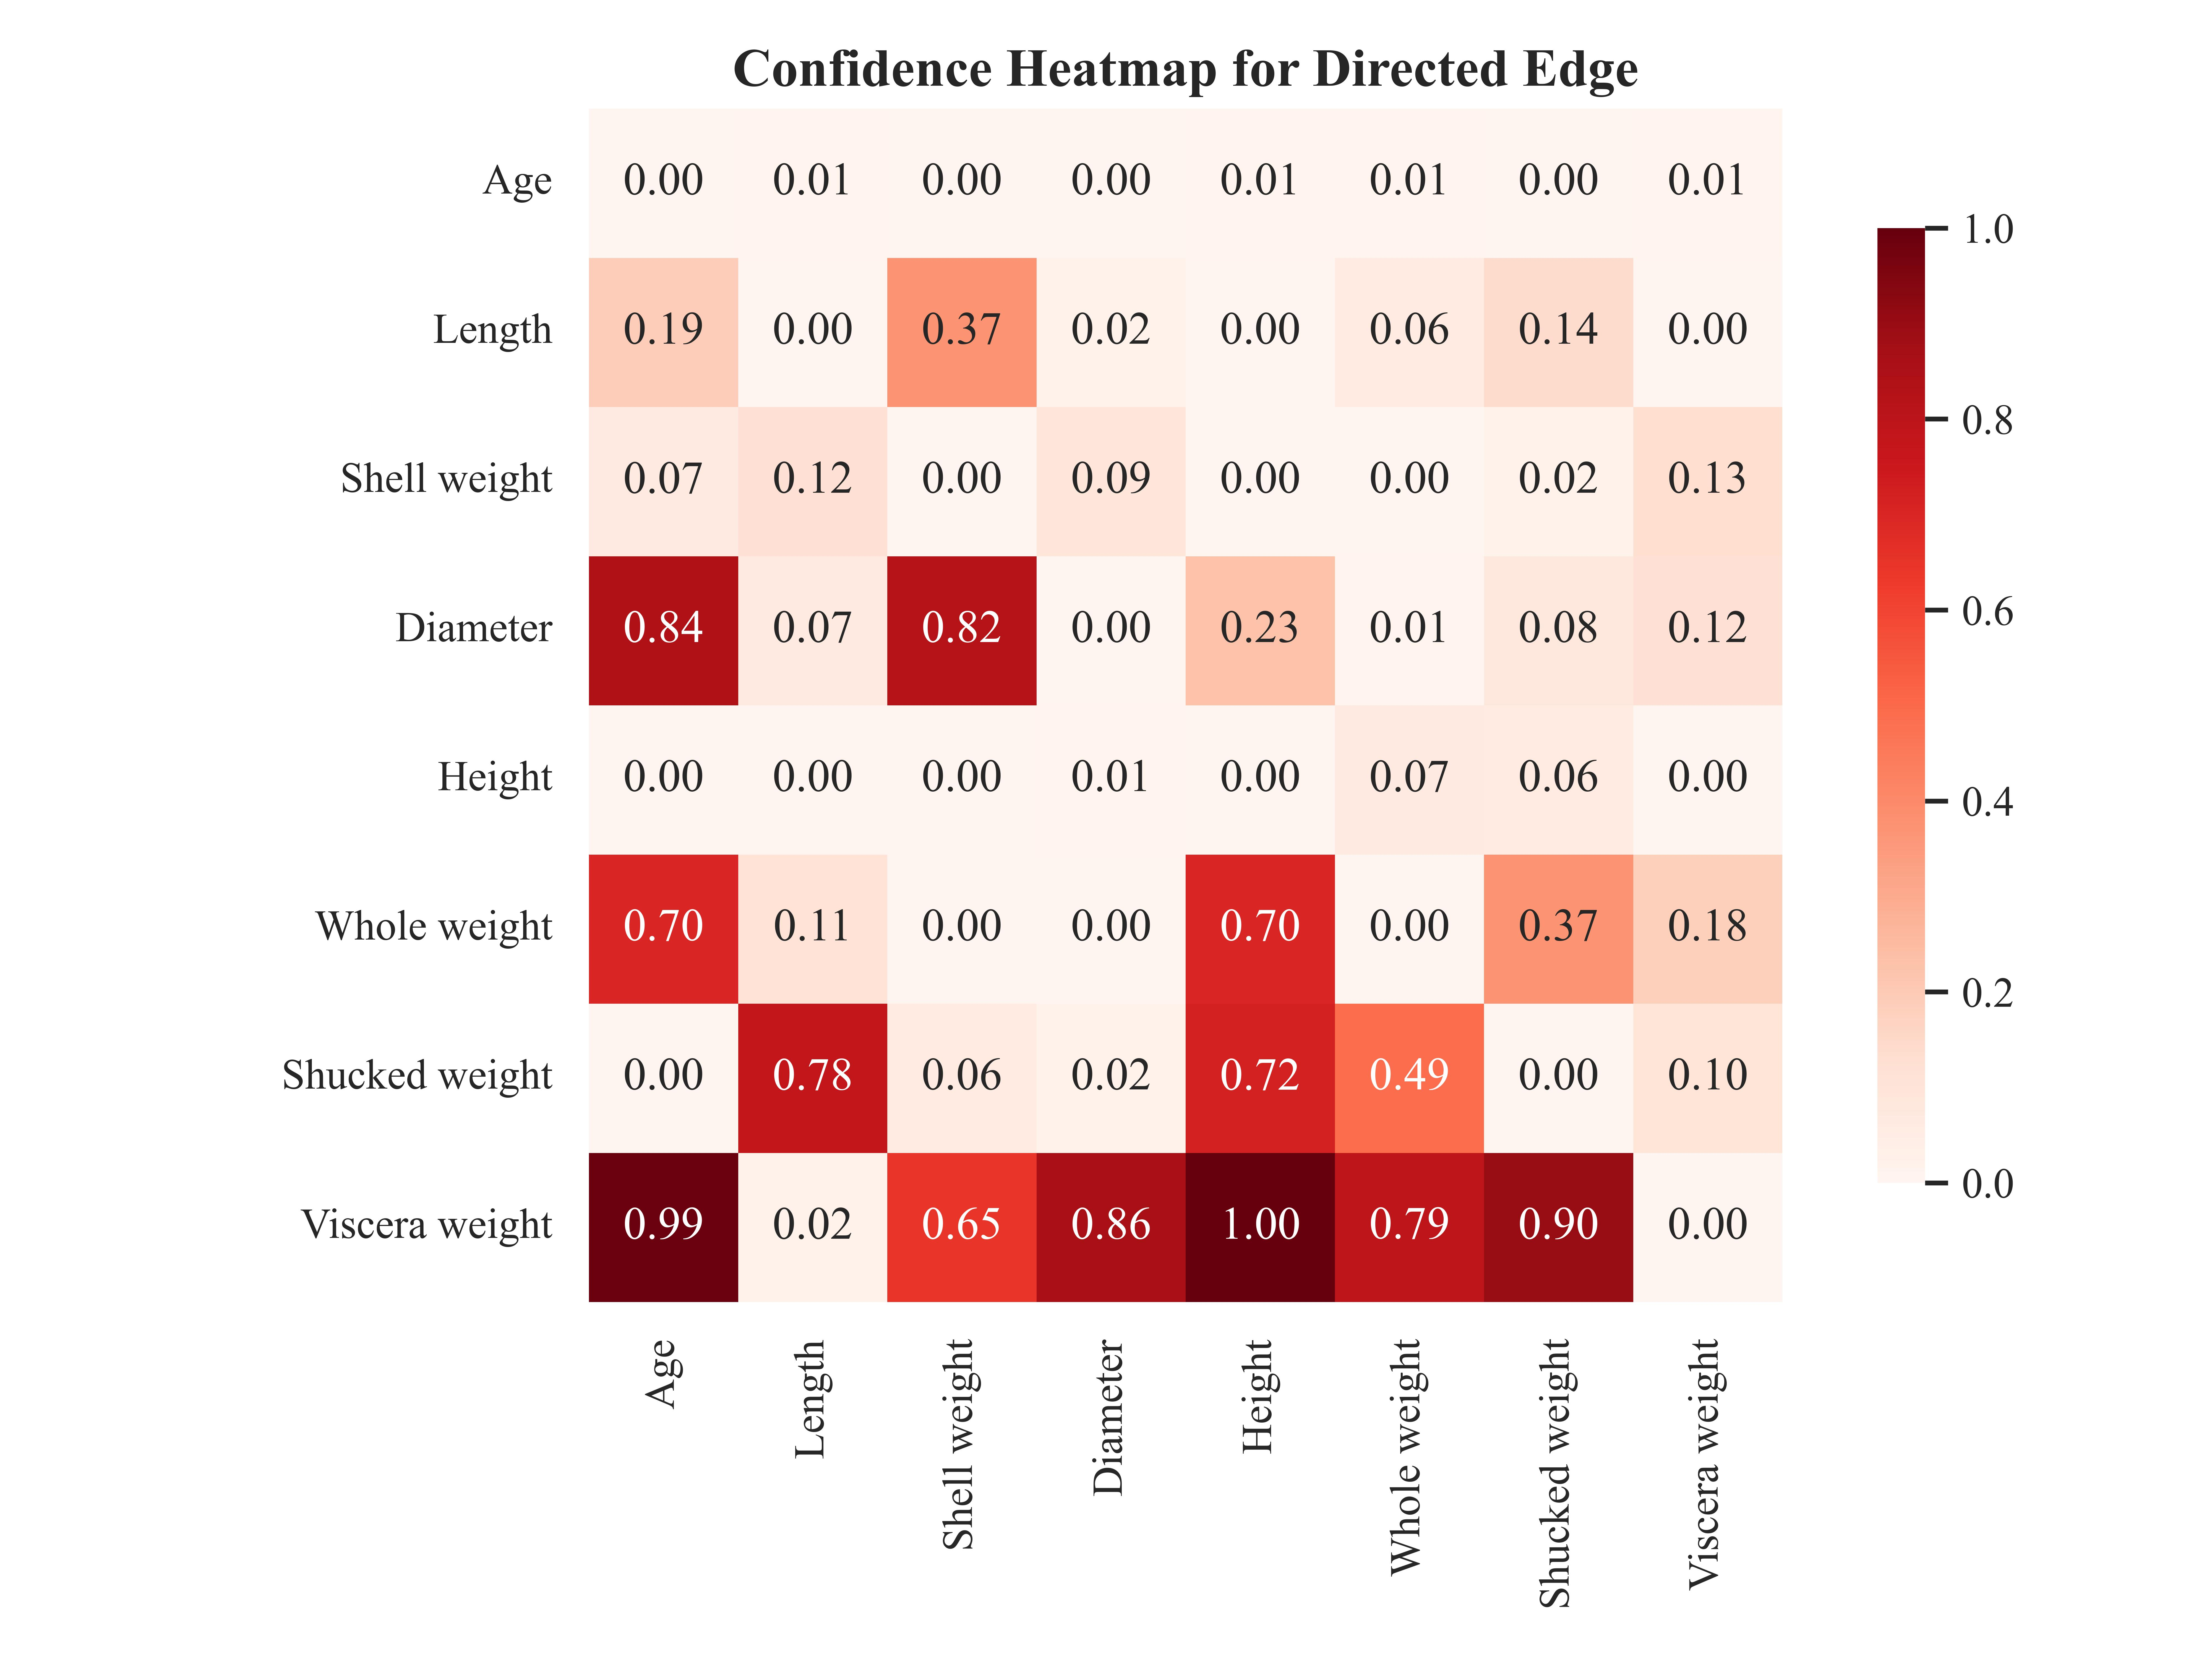
\includegraphics[width=\linewidth]{./demo_data/20241104_112841/Abalone/output_graph/certain_edges_confidence_heatmap.jpg}
        \caption{Directed Edge}
    \end{subfigure}
    \begin{subfigure}{0.32\textwidth}
        \centering
        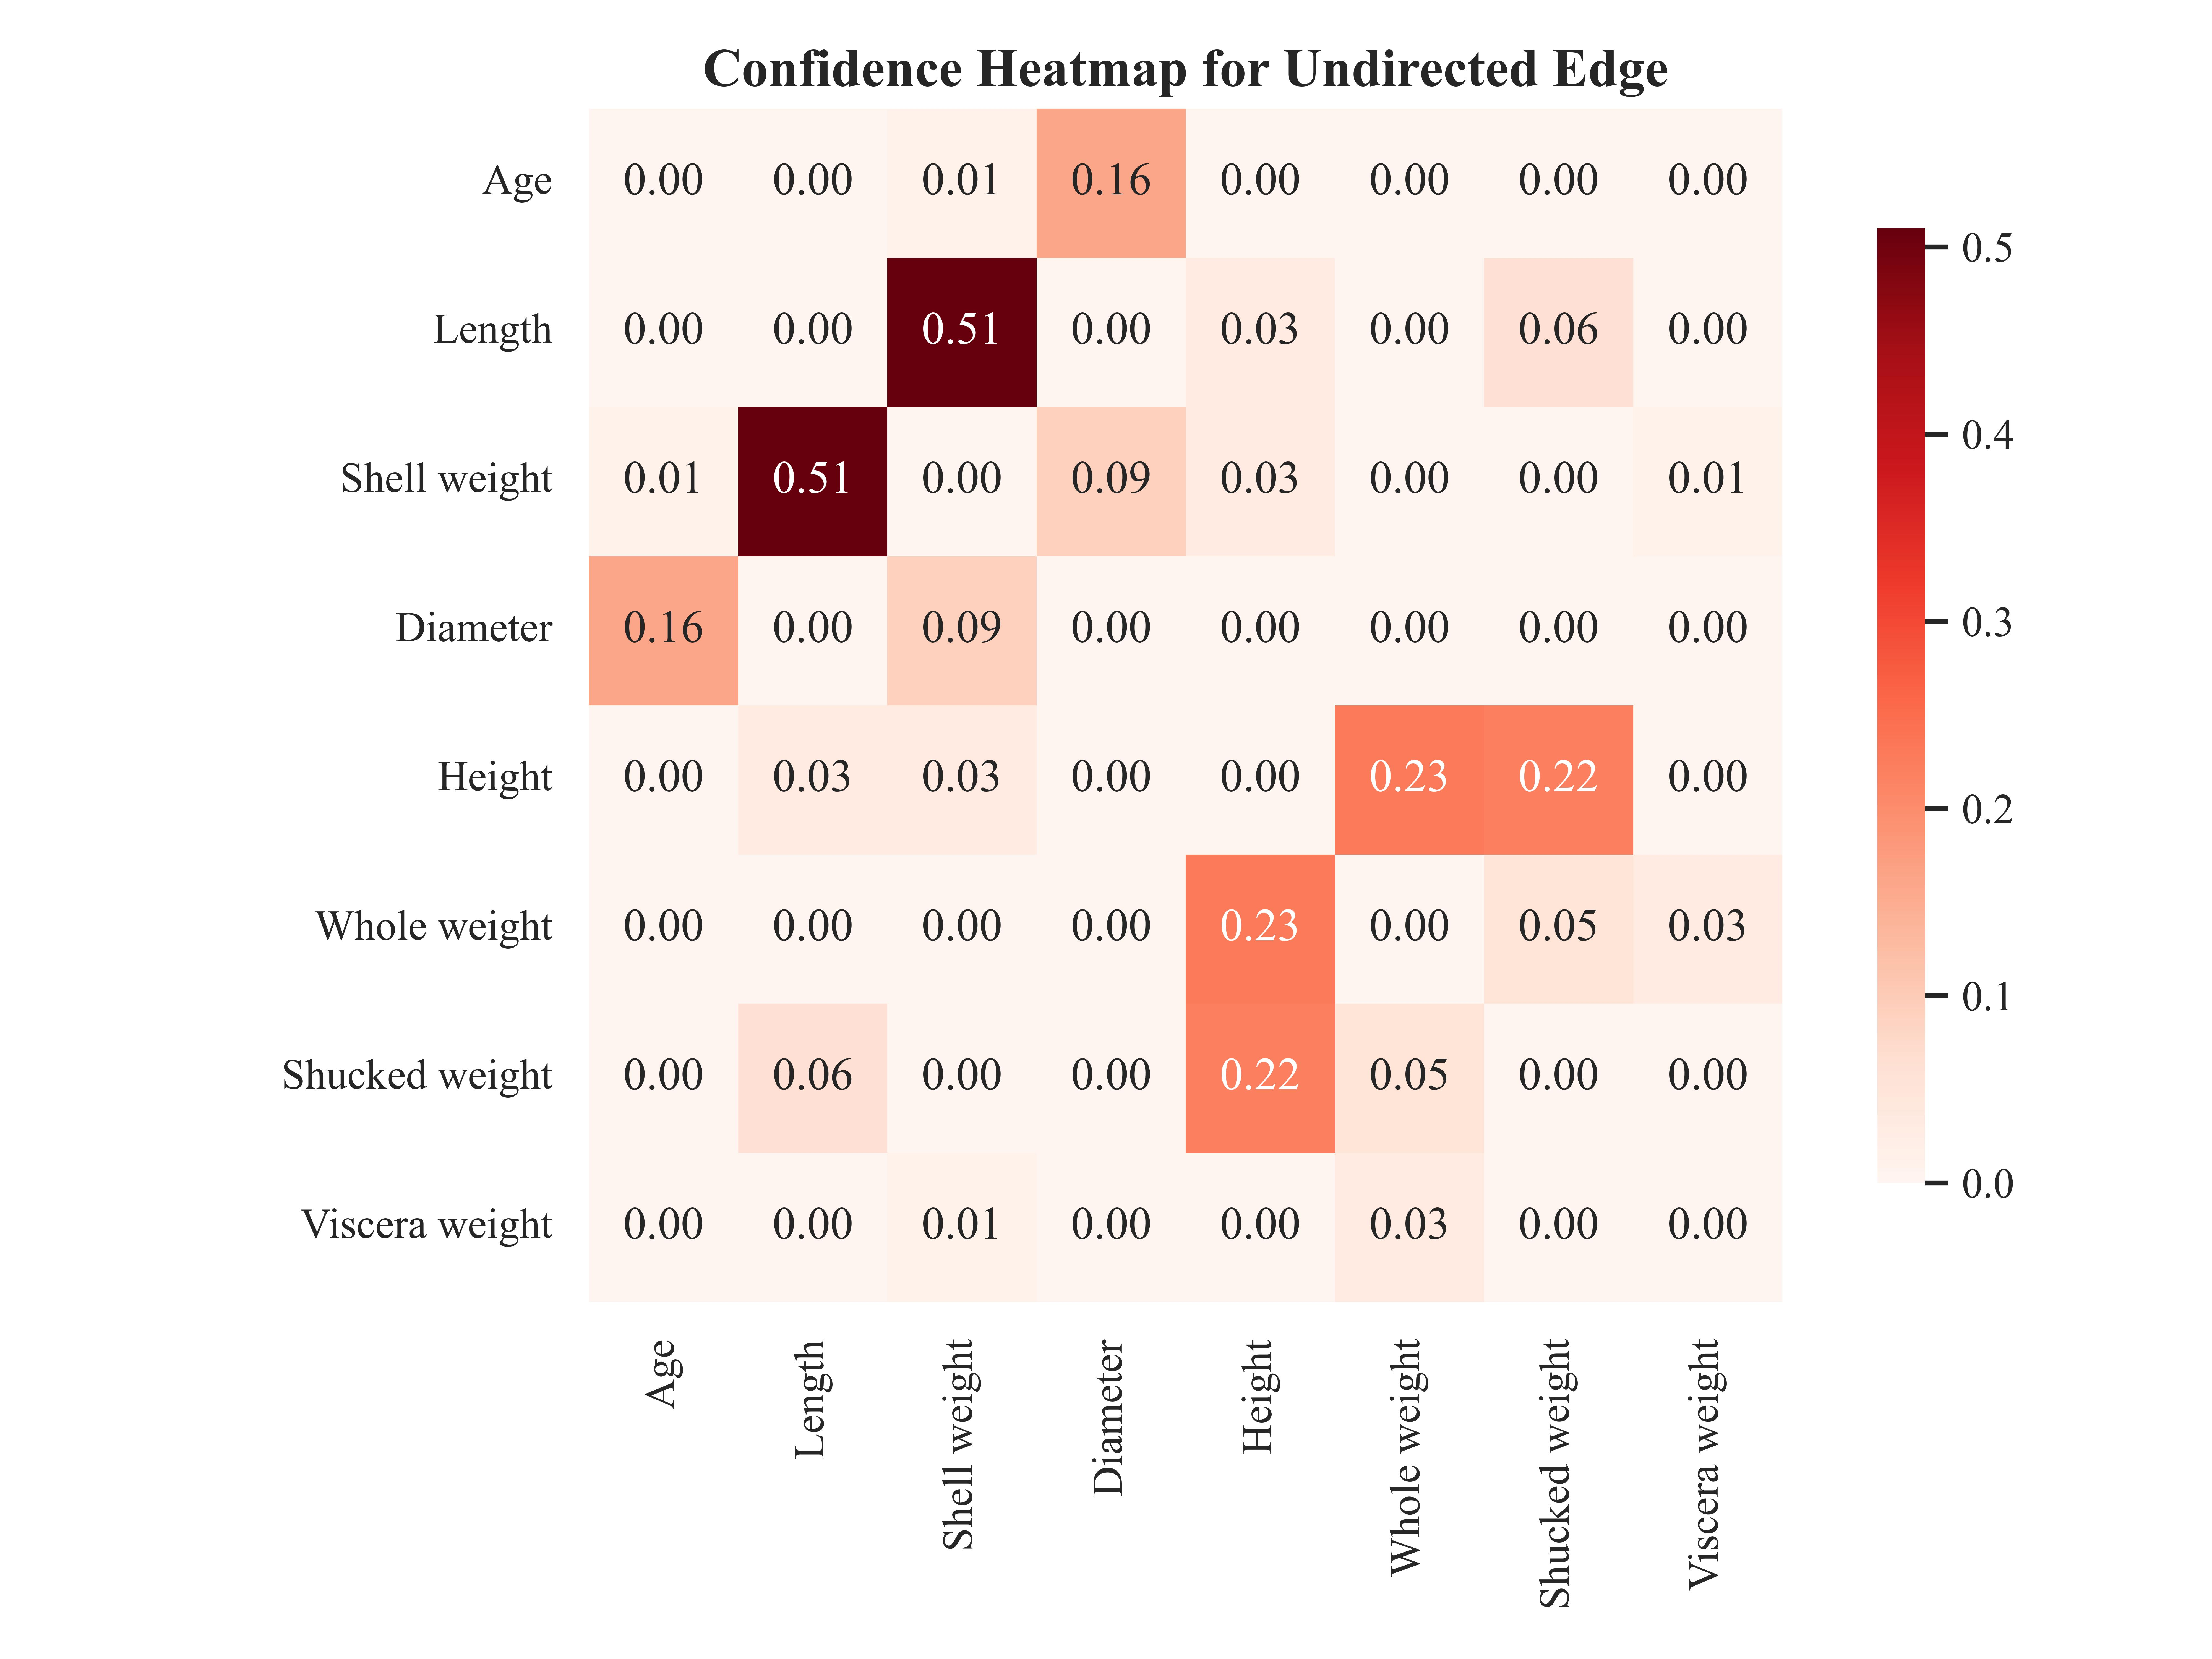
\includegraphics[width=\linewidth]{./demo_data/20241104_112841/Abalone/output_graph/uncertain_edges_confidence_heatmap.jpg}
        \caption{Undirected Edge}
    \end{subfigure}
    \begin{subfigure}{0.32\textwidth}
        \centering
        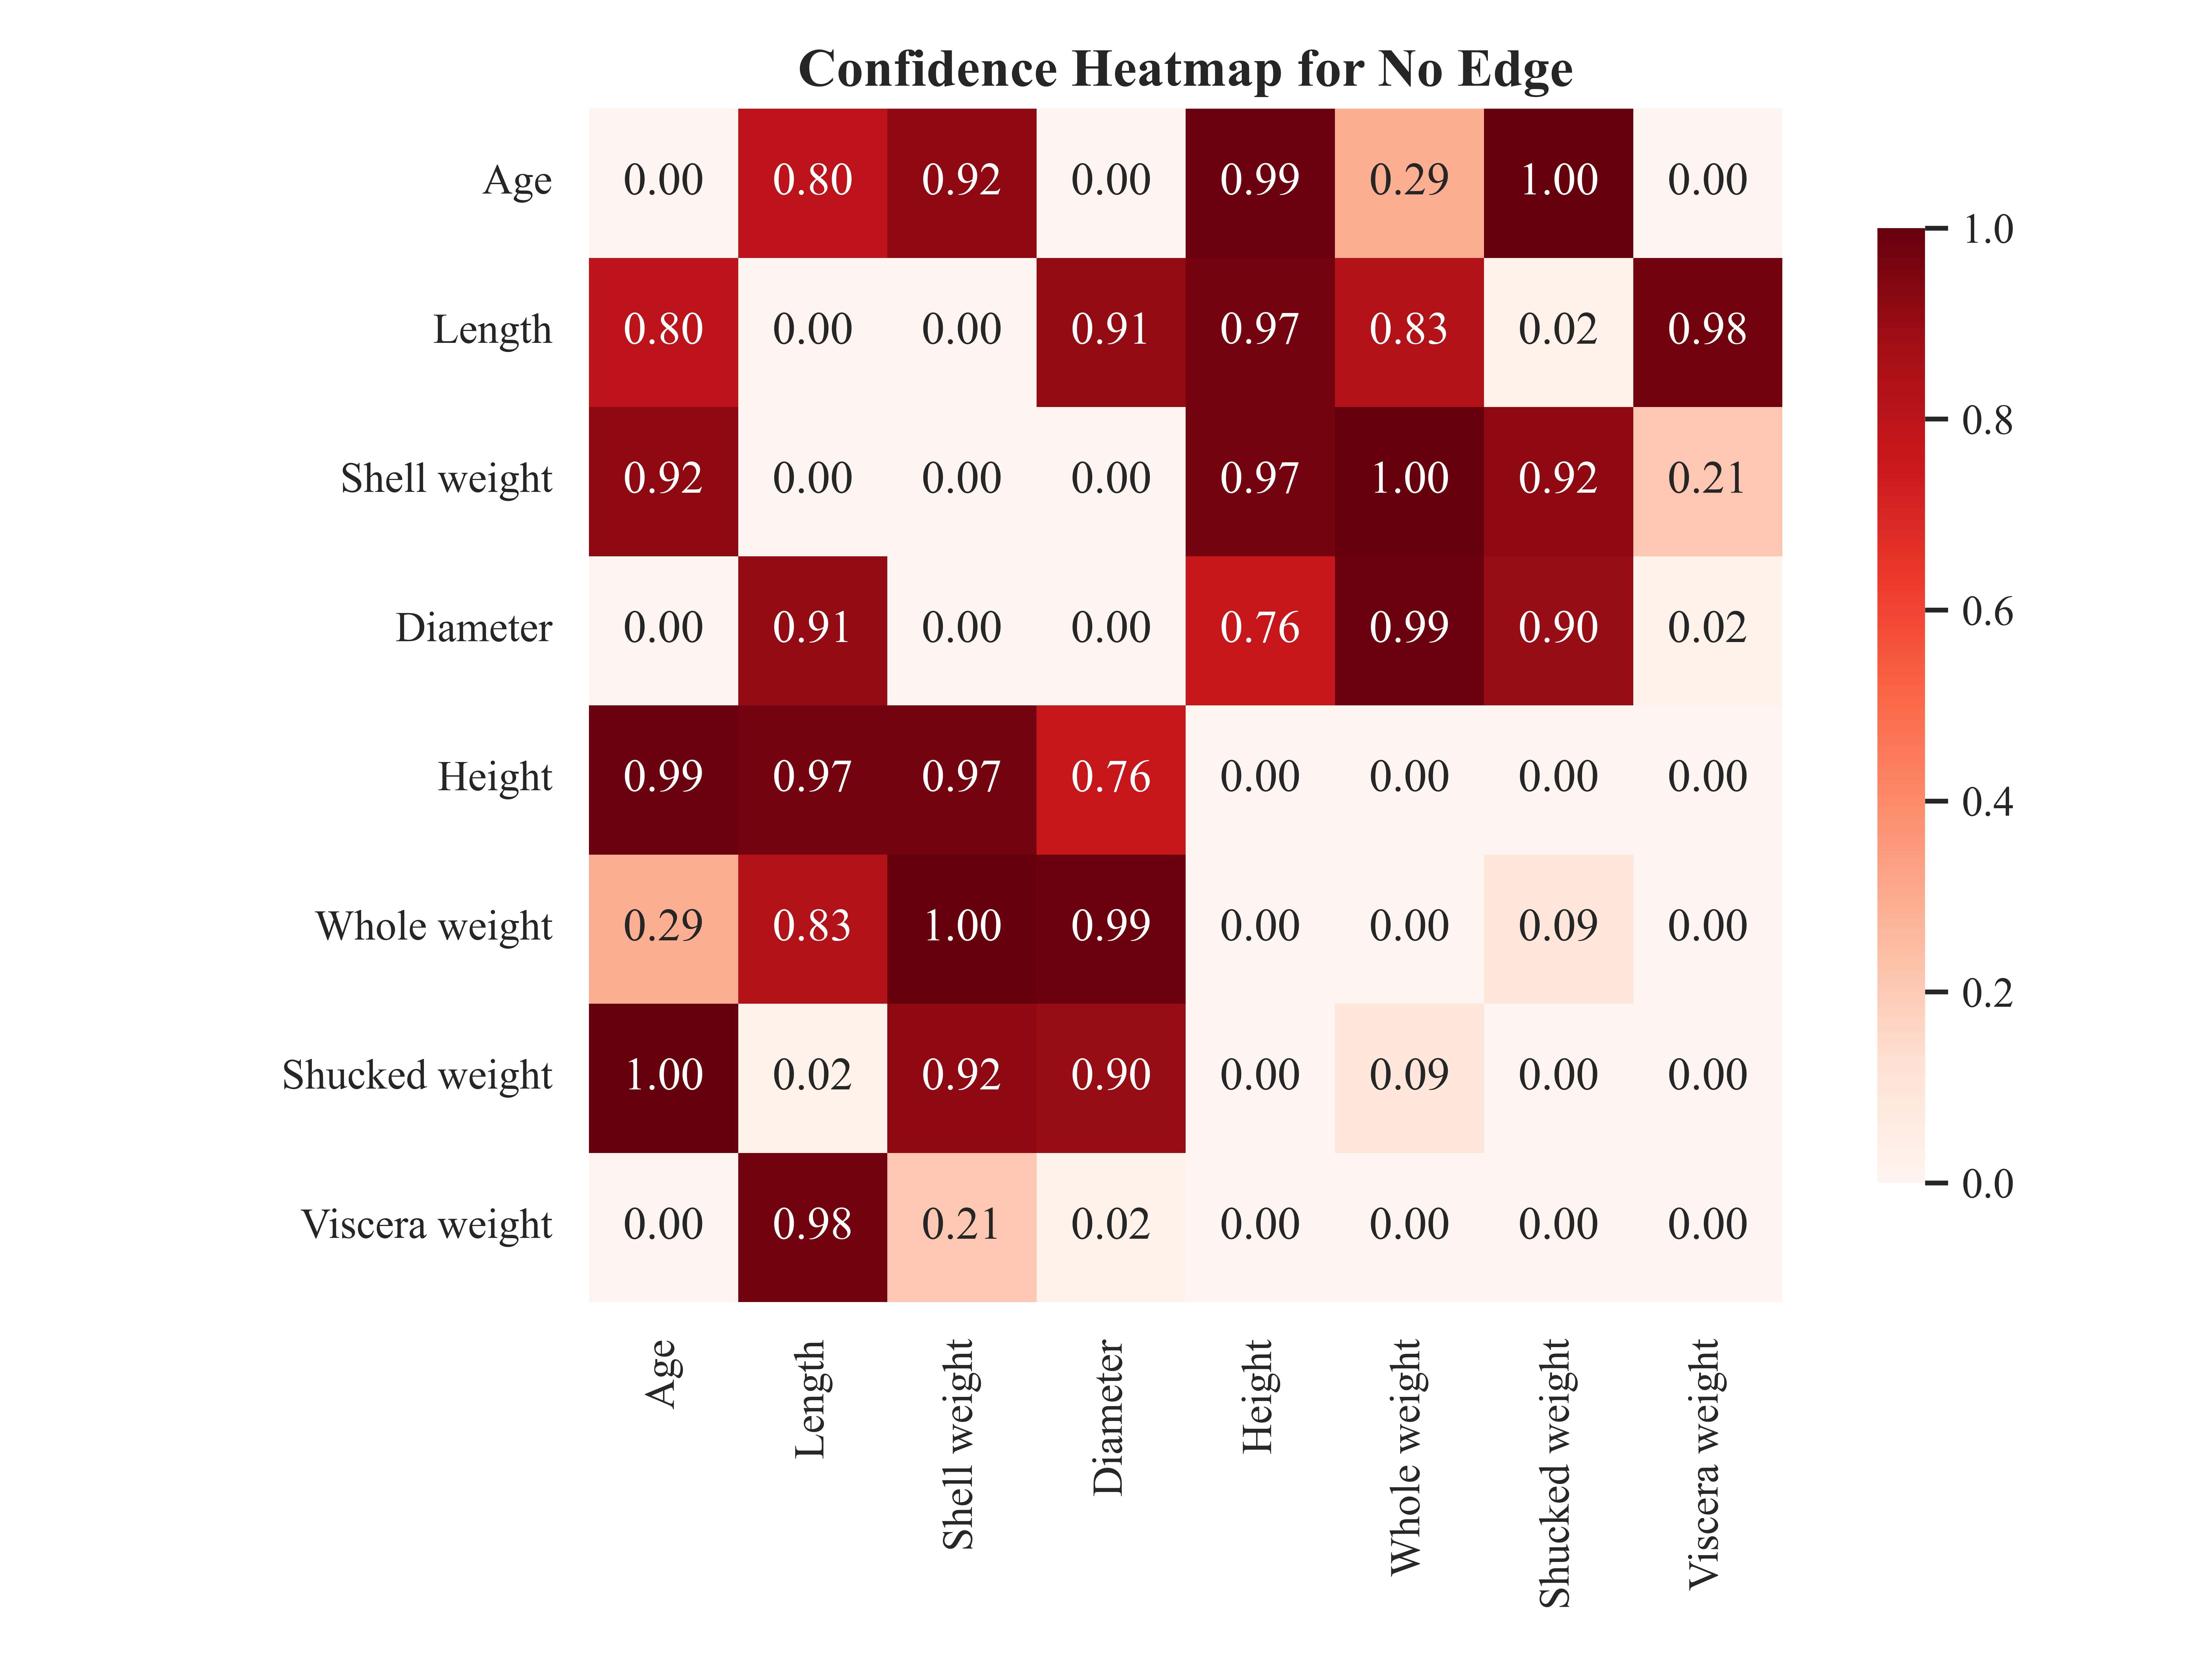
\includegraphics[width=\linewidth]{./demo_data/20241104_112841/Abalone/output_graph/non_existence_confidence_heatmap.jpg}
        \caption{No Edge}
    \end{subfigure}
    \caption{Confidence Heatmap of Different Edges}
\end{figure} 

The above heatmaps show the confidence probability we have on different kinds of edges, including directed edge ($\rightarrow$), undirected edge ($\leftrightarrow$), and no edge. The heatmap of bi-edges is not shown because probabilities of all edges are 0. Based on the confidence probability heatmap and background knowledge, we can analyze the reliability of our graph.

From the statistical perspective, we have high confidence to believe that these edges exist: \textbf{Whole weight $\rightarrow$ Height (0.7)} and \textbf{Whole weight $\rightarrow$ Shucked weight (0.37)}, while we have very low confidence in the edges \textbf{Age $\rightarrow$ Diameter (0.0)}, \textbf{Age $\rightarrow$ Viscera weight (0.01)}, and \textbf{Height $\rightarrow$ Diameter (0.01)}, indicating that these relationships are likely non-existent. However, based on expert knowledge, we know that these edges exist: \textbf{Age $\rightarrow$ Length}, \textbf{Age $\rightarrow$ Diameter}, and \textbf{Whole weight $\rightarrow$ Height}, as it is well-established that older abalones grow larger in physical dimensions and overall weight. We also recognize that some edges such as \textbf{Length $\rightarrow$ Shell weight} and \textbf{Shell weight $\rightarrow$ Viscera weight} may have more relevance because the weight of the shell contributes to the overall weight and growth metrics of the abalone. Therefore, the result of this causal graph is not entirely reliable. While some statistical edges show potential, the lack of strong evidence for several key relationships from a biological standpoint indicates a need for caution in interpreting these causal links.

\end{document}